\documentclass[aspectratio=169, handout]{beamer}
\usepackage[utf8]{inputenc}
\usepackage{amsmath}
\usepackage{tikz}
\usepackage{pgfplots}
\usepackage{dsfont}
\usepackage{opensans}

\usetheme{NOVASBE}

\title[]{4509 - Bridging Mathematics}
\subtitle{Differential Equations\\ and Phase Diagrams}
\author[P. Fagandini]{Paulo Fagandini}
\institute{}
\date{}

\makeatother

\newtheorem{defenition}{Definition}[section]
\newtheorem{proposition}{Conjecture}[section]

\begin{document}

\begin{frame}{Differential Equations}

Often we have a variable that depends on time:

\begin{itemize}
    \item $x_t$ in discrete models
    \item $x(t)$ in continuous models
\end{itemize}

This variable reflects the state of a system at the point in time $t$. Let $x_t,x(t)\in X \subseteq \mathds{R}^n$. This is called the \textbf{state vector}.
    
\end{frame}

\begin{frame}{Differential Equations}
    The \textbf{state vector} reflects the state of the system (for example the economy), and it is interesting to understand how this state changes over time.
    
    In this environment, the state of the system will depend on the \textbf{initial condition} (\(x_0)\), the period (\(t\in\mathds{R}\)), and the parameters of the system (\(\theta\in\Theta\subseteq\mathds{R}^p\)).
    
    Then we can define the function \emph{flow}:
    \[\phi:X\times\mathds{R}_+\times\Theta\rightarrow \mathds{R}^n\] \[x_t=\phi(x_0,t,\theta)\]
\end{frame}

\begin{frame}{Differential Equations}

    $\phi$ describes the system for every period, given the initial state and parameters, and therefore, replacing $t$ for every period of our interest, we can pin down the state of the system.
    
    Usually the challenge is to find $\phi$ from an initial system of differential equations.
    
\end{frame}

\begin{frame}{Differential Equation}
    \begin{definition}
        An ordinary \textbf{differential equation} is an equation of the form \[x^{(m)}(t)=F[t,x(t),\dot{x}(t),\ddot{x}(t),\ldots,x^{(m-1)}(t),\theta]\]
        Where \(x(t)=[x_1(t),x_2(t),\ldots,x_n(t)]\) is a vector-valued function of a real variable that we will interpret as time $(t)$, and
        \[\dot{x}(t)=\left[\frac{d x_1(t)}{dt},\frac{d x_2(t)}{dt},\ldots,\frac{d x_n(t)}{dt}\right]\]
        is the first derivative of $x(t)$ with respect to time, and $\ddot{x}(t)$ is the second derivative and $x^{(m)}$ its mth derivative, \(\theta\in\Theta\subseteq\mathds{R}^p\) is a vector of parameters, and $F(\cdot)$ is a function $\mathds{R}^{1+n(m-1)+p}\rightarrow\mathds{R}^n$ that is typically assumed to be at least once differentiable.
    \end{definition}
\end{frame}

\begin{frame}{Differential Equation}
    The solution to this differential equation, is to find a function $x(t)$ such that along with its derivatives with respect to time \[x^{(m)}(t)=F[t,x(t),\dot{x}(t),\ddot{x}(t),\ldots,x^{(m-1)}(t),\theta]\] is satisfied.
    
    \vspace{0.5cm}
    
    In the case of working in a discrete environment, $x_t$ is a sequence instead of a function $x(t)$. We just saw a basic example within a discrete environment, but the whole analysis will now focus on continuous environments (looks harder, but it is easier...)
\end{frame}

\begin{frame}{Differential Equation}
    \begin{definition}
        A differential equation is \textbf{linear} if $F(\cdot)$ is linear in $x(t)$ and its derivatives, but not necessarily in $t$ or $\theta$.
    \end{definition}
    \begin{definition}
        A dynamical system is \textbf{autonomous} if $t$ does not appear as an independent argument of $F(\cdot)$ but enters only through $x(t)$ and derivatives.
    \end{definition}
\end{frame}

\begin{frame}{Differential Equation}
    A system being linear or not has huge implications. For linear systems it is in general possible to find an analytical solution, while for nonlinear solutions in general you need to use numerical solutions (particular instead of general) or do only qualitative analysis.
    
    \vspace{0.5cm}
    
    For non linear autonomous systems of one or two dimensions, qualitative results can be obtained easily with graphical representations. For higher dimensions, it is necessary to rely on linear approximations.
    
\end{frame}

\begin{frame}{Differential Equation}
    \begin{definition}
    The \textbf{order} of a differential equation is the order of the highest derivative of $x(t)$ that appears on it.
    \end{definition}
    \begin{fact}
        Any system of differential equations can be reduced to an equivalent first-order system by introducing additional equations and variables.
    \end{fact}
\end{frame}

\begin{frame}{Differential Equation}
    \begin{example}
        Consider the second-order differential equation
        \[\ddot{x}(t)=a \dot{x}(t)+bx(t)\]
        Let \(y(t)=\dot{x}(t)\),
        \[\dot{y}(t)=a y(t)+bx(t)\quad \text{and}\quad \dot{x}(t)=y(t)\]
    \end{example}
    
    In conclusion, without loss of generality we restrict our analysis first order systems of differential equations of the form: \[\dot{x}(t)=f(x(0),t,\theta)\]
    
\end{frame}

\begin{frame}{Geometrical Interpretation}
    \begin{center}
        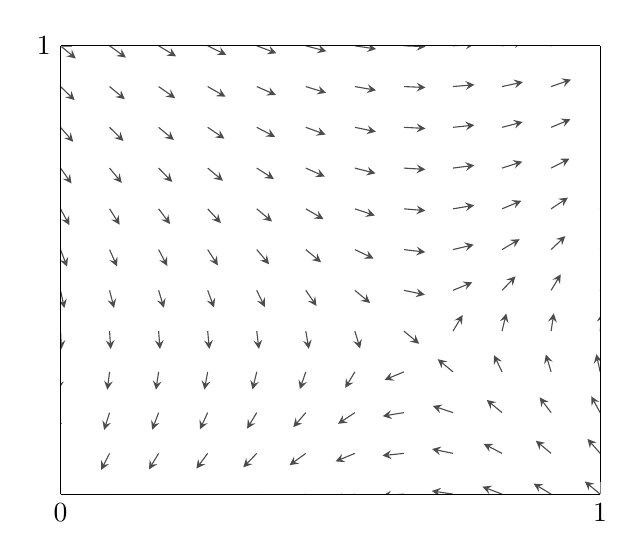
\begin{tikzpicture}
            \begin{axis}[domain=0:1, xmin=0, xmax=1, ymin=0, ymax=1, 
            xtick pos=bottom, ytick pos=left, 
            xlabel style={anchor=west,at={(1,-0.1)},xshift=10pt}, 
            xtick={0,1}, xticklabels={0,$1$},
            ylabel style={anchor=south,at={(-0.1,1)},yshift=1mm,rotate=-90},
            ytick={1}, yticklabels={1}, view={0}{90} 
            ]
                \addplot3[color=black!70!white,
                    quiver={
                        u={(y-1/3)/veclen(x-2/3,y-1/3)},
                        v={(x-2/3)/veclen(x-2/3,y-1/3)},
                        scale arrows=0.04,
                    },
                    -stealth,
                    samples=12]{0};
                \path (0,0,0) coordinate (P1) (1,1,0) coordinate (P2)
                 (2/3,1/3,0) coordinate (P3);

            \end{axis}
        \end{tikzpicture}
    \end{center}
\end{frame}

\begin{frame}{Differential Equations}

So as we see, we can find $\phi(x_0,t,\theta)$, but this is not unique! it depends on the initial value we choose. This is why this could be called \textbf{general solution}. To pin down a \textbf{particular solution}, a traditional way is to fix the initial value of $x_0$ or $x(t=0)$, the starting point. Note however that we could have fixed $x(1)$ or more generally $x(\hat{t})$ with the same effect. If we can obtain $x(t)$ from $x(0)$, we can get $x(0)$ from $x(t)$!
    
\end{frame}

\begin{frame}{Differential Equations}
    Consider the continuous system \begin{align}\dot{x}(t)=f(x,\theta,t)\label{eq:def1}\end{align} where $f:X\times\Theta\times I\rightarrow X$, and $I\subseteq\mathds{R}$ compact and convex.
    \begin{definition}
        A \textbf{\textit{particular} solution} of \eqref{eq:def1} is a differentiable function $\phi(t):J_{\phi}\rightarrow X$, defined on some interval $J_{\phi}\subseteq I$ called its \textbf{interval of definition}, and taking values in $X$, that together with its derivative satisfies the differential equation \eqref{eq:def1} in $J_\phi$, that is such that \[\phi'(t)=f[\phi(t),\theta,t]\forall t\in J_\phi\]
    \end{definition}
\end{frame}

\begin{frame}{Differential Equations}
    \begin{definition}
        Given a solution $\phi(t)$ of the differential equation \eqref{eq:def1} defined on the interval $J_\phi$, we define the \textbf{orbit} of \eqref{eq:def1} induced by $\phi$ as the set \[\gamma(\phi)=\phi(J_\phi)=\{x\in X; x=\phi(t)\ \text{for some}\ t\in J_\phi\}\]
    \end{definition}
    
\end{frame}

\begin{frame}{Differential Equations}

\begin{theorem}
     Let $f:X\times I\times\Theta\subseteq\mathds{R}^{n+p+1}\rightarrow\mathds{R}^n$ be (at least) once differentiable on the set $X\times I\times \Theta$, where $X$ and $\Theta$ are open sets, and $I$ is an interval in the real line. Then the boundary-value problem \[\dot{x}=f(x,\theta,t),\ x(t_0)=x_0\] has unique solution $\phi(t)=\phi(t,x_0,t_0,\theta)$ for each $(x_0,t_0,\alpha)\in X\times I\times\Theta$ defined on a maximal open interval $J_m=(x_0,t_0,\alpha)\subseteq I$ containing $t_0$ that depends on the initial data and parameters of the problem. That is, if $\Psi(t)$ is a solution defined on some interval $J_\Psi$, then $J_\psi\subseteq J_m(x_0,t_0,\theta)$ and $\Psi(t)=\phi(t)$ for all $t\in J_\psi$. Moreover, the flow of the system, $\phi(t,x_0,t_0,\alpha)$ is at least once differentiable. 
\end{theorem}
    
\end{frame}

\begin{frame}{Example}

Consider the system \[\dot{x}=f(x)=3x^{2/3}\ \text{and,}\ x(0)=0\]

\begin{enumerate}
    \item<2-> Rewrite \[\dot{x}=\frac{dx}{dt}=3x^{2/3}\]
    \item<3-> Rearrange \[dt=\frac{x^{-2/3}}{3}dx\]
    \item<4-> Integrate both sides \[\int dt = \int \frac{x^{-2/3}}{3}dx\Rightarrow c+t=x^{1/3}\]
\end{enumerate}
    
\end{frame}

\begin{frame}{Example}
    So the functions of the form \[x(t)=(c+t)^3\] are solutions of the given differential equation. Now, note the initial condition $x(0)=0$,
    \[x(0)=(c+0)^3\Rightarrow 0=c^3\Rightarrow c=0\]
    Finally, \[x(t)=t^3\]
\end{frame}

\begin{frame}{Phase Diagrams}

    Consider the following system of equations in the plane:
    \begin{align*}
        \dot{x}=f(x,y)\\
        \dot{y}=g(x,y)
    \end{align*}
    With $f$ and $g$ differentiable.
    
    Set $\dot{x}$ and $\dot{y}$ equal to zero. This finds the region where these variables do not change over time, these lines are called \textbf{phase lines}.
    
    \begin{align*}
        \dot{x}=0\Rightarrow f(x,y)=0\\
        \dot{y}=0\Rightarrow g(x,y)=0
    \end{align*}
    
\end{frame}

\begin{frame}{Phase Diagrams}
    \begin{columns}
        \begin{column}{0.47\textwidth}
            The phase line $\dot{x}=0$ divides the $(x,y)$ plane into two regions.
            \begin{enumerate}
                \item In one of them $\dot{x}>0$, so $x\uparrow$,
                \item  and the other $\dot{x}<0$ so $x\downarrow$.
            \end{enumerate}
        \end{column}
        
        \pause

        \begin{column}{0.47\textwidth}
            \begin{center}
                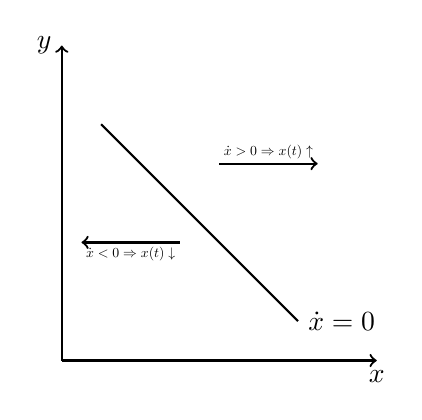
\begin{tikzpicture}
                    \draw[->,thick] (0,0)--(4,0)node[below]{$x$};
                    \draw[->,thick] (0,0)--(0,4)node[left]{$y$};
                    
                    \draw[thick] (0.5,3)--(3,0.5)node[right]{$\dot{x}=0$};
                    \draw[thick,->] (1.5,1.5)--(0.25,1.5)node[midway,below,scale=0.5]{$\dot{x}<0\Rightarrow x(t)\downarrow$};
                    \draw[thick,->] (2,2.5)--(3.25,2.5)node[midway,above,scale=0.5]{$\dot{x}>0\Rightarrow x(t)\uparrow$};
                    
                \end{tikzpicture}
            \end{center}
        \end{column}
    \end{columns}
\end{frame}

\begin{frame}{Phase Diagrams}
    \begin{columns}
        \begin{column}{0.47\textwidth}
            The phase line $\dot{y}=0$ divides the $(x,y)$ plane into two regions.
            \begin{enumerate}
                \item In one of them $\dot{y}>0$, so $y\uparrow$,
                \item and the other $\dot{y}<0$ so $y\downarrow$.
            \end{enumerate}
        \end{column}

        \begin{column}{0.47\textwidth}
            \begin{center}
                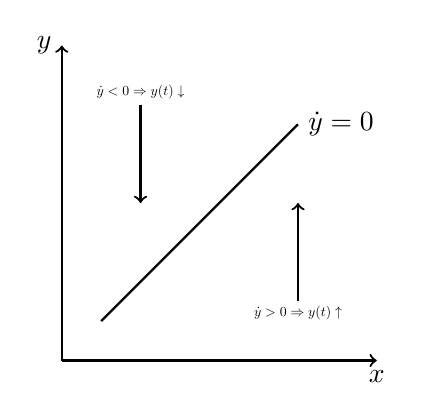
\begin{tikzpicture}
                    \draw[->,thick] (0,0)--(4,0)node[below]{$x$};
                    \draw[->,thick] (0,0)--(0,4)node[left]{$y$};
                    
                    \draw[thick] (0.5,0.5)--(3,3)node[right]{$\dot{y}=0$};
                    
                    \draw[thick,->] (1,3.25)node[above,scale=0.5]{$\dot{y}<0\Rightarrow y(t)\downarrow$}--(1,2);
                    \draw[thick,->] (3,0.75)node[below,scale=0.5]{$\dot{y}>0\Rightarrow y(t)\uparrow$}--(3,2);
                    
                \end{tikzpicture}
            \end{center}
        \end{column}
    \end{columns}
\end{frame}

\begin{frame}{Phase Diagrams}
    
    The direction in which the large arrows are pointing (and for the sake of the argument the phase lines too) could seem arbitrary, and they are, just an example.\pause
    
    To determine in which side of the phase line the variable increases or decreases we could evaluate their derivatives:
    \[\frac{\partial\dot{x}}{\partial x}=\frac{\partial f(x,y)}{\partial x}\quad \frac{\partial\dot{y}}{\partial y}=\frac{\partial f(x,y)}{\partial y}\]
    Then evaluate it at a convenient point, say a point in the phase line. If the derivative is positive, this means it increases, and therefore to the right it will be increasing even further. The opposite is true if the derivative is negative.
\end{frame}

\begin{frame}{Phase Diagrams}
    \begin{columns}
        \begin{column}{0.47\textwidth}
            \begin{center}
                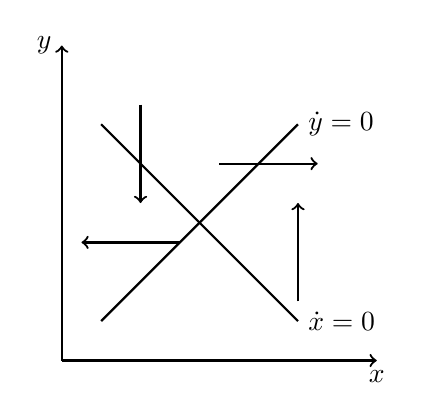
\begin{tikzpicture}
                
                    \draw[->,thick] (0,0)--(4,0)node[below]{$x$};
                    \draw[->,thick] (0,0)--(0,4)node[left]{$y$};
                    
                    \draw[thick] (0.5,0.5)--(3,3)node[right]{$\dot{y}=0$};
                    \draw[thick,->] (1,3.25)--(1,2);
                    \draw[thick,->] (3,0.75)--(3,2);
                    
                    \draw[thick] (0.5,3)--(3,0.5)node[right]{$\dot{x}=0$};
                    \draw[thick,->] (1.5,1.5)--(0.25,1.5);
                    \draw[thick,->] (2,2.5)--(3.25,2.5);
                    
                \end{tikzpicture}
            \end{center}
        \end{column}
        \pause
        \begin{column}{0.47\textwidth}
            \begin{center}
                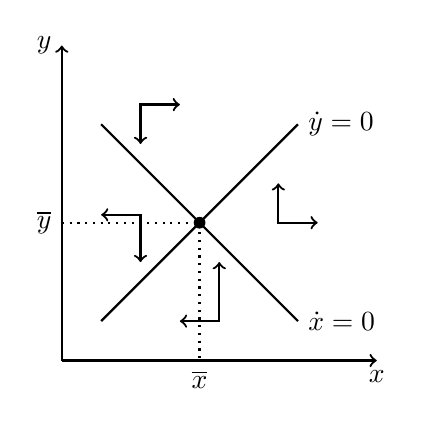
\begin{tikzpicture}
                
                    \draw[->,thick] (0,0)--(4,0)node[below]{$x$};
                    \draw[->,thick] (0,0)--(0,4)node[left]{$y$};
                    
                    \draw[thick] (0.5,0.5)--(3,3)node[right]{$\dot{y}=0$};
                    
                    \draw[thick,<->] (1.5,3.25)--(1,3.25)--(1,2.75);
                    \draw[thick,<->] (1.5,0.5)--(2,0.5)--(2,1.25);
                    
                    \draw[thick] (0.5,3)--(3,0.5)node[right]{$\dot{x}=0$};
                    \draw[thick,<->] (1,1.25)--(1,1.85)--(0.5,1.85);
                    \draw[thick,<->] (2.75,2.25)--(2.75,1.75)--(3.25,1.75);
                    
                    \draw[dotted,thick] (0,1.75)node[left]{$\overline{y}$} -- (1.75,1.75) node[circle,fill,inner sep=1.5]{} -- (1.75,0)node[below]{$\overline{x}$};
                    
                \end{tikzpicture}
            \end{center}
        \end{column}
    \end{columns}
    $(\overline{x},\overline{y})$ is a steady state of the system, note that at this point $\dot{x}=0$ and $\dot{y}=0$.
\end{frame}

\begin{frame}{Local Analysis by Linearization}

Let $f:x\subseteq\mathds{R}^n\rightarrow \mathds{R}^n$, differentiable, and $x_0\in X$. By the Taylor expansion we can write:
\begin{align*}
    f(x)=f(x_0)+Df(x_0)(x-x_0)+E_f(x-x_0)
\end{align*}
    with $\lim_{x\rightarrow x_0} \frac{||E_f(x-x_0)||}{||x-x_0||} = 0$. Consider also a nonlinear autonomous system \[\dot{x}=f(x)\]
    And let $\overline{x}$ be a steady state of the system, then the linear system \[\dot{x}=Df(\overline{x})(x-\overline{x})\] can be expected to be a reasonable approximation of the original system around the equilibrium point $\overline{x}$.
\end{frame}

\begin{frame}{Local Analysis by Linearization}
\begin{theorem}
    Consider the system $\dot{x}=f(x)$, where $f:X\subseteq\mathds{R}^n\rightarrow\mathds{R}^n$, differentiable, and let $\overline{x}$ be an equilibrium point of the system. The the following holds:
    \begin{enumerate}
        \item If all eigenvalues of $Df(\overline{x})$ have strictly negative real parts, then $\overline{x}$ is asymptotically stable.
        \item If at least one eigenvalue of $Df(\overline{x})$ has a positive real part, then $\overline{x}$ is (locally) unstable.
        \item If at least one eigenvalue of $Df(\overline{x})$ has a zero real part, and all other eigenvalues have negative real parts, then the equilibrium $\overline{x}$ might be stable, asymptotically stable, or unstable.
    \end{enumerate}
\end{theorem}
    
\end{frame}

\begin{frame}{Example}
    Consider the following system of differential equations:
    \begin{align}
        \dot{x}=f(x,y)=y+x(c-x^2-y^2)\label{ex1a}\\
        \dot{y}=g(x,y)=-x+y(c-x^2-y^2)\label{ex1b}
    \end{align}
\end{frame}

\begin{frame}{Example}
    Let's show that $(0,0)$ is the only solution (i.e. $\dot{x}=0$ and $\dot{y}=0$)
    \begin{enumerate}
        \item Obviously $(0,0)$ is a solution, as if we replace $(0,0)$ we obtain $\dot{x}=0$ and $\dot{y}=0$.
        \item If one of them is zero, then the other must be zero too! (let $y=0$, then $\dot{y}=-x$, but in equilibrium we need $\dot{y}=0$ so $x=0$, idem for the case $x=0$).
        \item Let $x,y\neq0$, then we can divide \eqref{ex1a} and \eqref{ex1b} by $x$ and $y$ respectively, and obtain
        \begin{align*}
            \frac{-y}{x}=c-x^2-y^2\\
            \frac{x}{y}=c-x^2-y^2\\
        \end{align*}
        But that means $\frac{-y}{x}=\frac{x}{y}$ or $-y^2=x^2$, which is only true for $x=y=0$, contradiction!
    \end{enumerate}
\end{frame}
\begin{frame}{Example}
    Now let's linearize the system, find its eigenvalues and study the stability around the steady state $(0,0)$, let's see what can we say about it.
    
    \pause
    
    The partial derivatives of $f$ and $g$, at $(0,0)$, are:
    \begin{align*}
        f_x(0,0)=c\\
        f_y(0,0)=1\\
        g_x(0,0)=-1\\
        g_y(0,0)=c
    \end{align*}
    
\end{frame}

\begin{frame}{Example}
    The coefficient matrix of the linearized system is of the form (Jacobian): \[A=\begin{bmatrix}c&1\\-1&c\end{bmatrix}\] finding the eigenvalues we solve \(|A-\lambda I|=0\) or the characteristic polynomial \[(c-\lambda)^2+1=0\] and therefore $c-\lambda = \pm i$ or $\lambda = c\pm i$. $c$ is the real part of the eigenvalue, and using the theorem we had about stability we can say:
    \begin{enumerate}
        \item If $c<0$ the steady state is locally stable.
        \item If $c>0$ the steady state is locally unstable.
        \item If $c=0$ we cannot say much with the available information.
    \end{enumerate}
\end{frame}

\end{document}
